\chapter{Architecture and Implementation}
\label{ch:architecture-and-implementation}

\section{Third-Party Tools}
\label{sec:third-party-tools-architecture}

\subsection{Docker}
\label{sec:docker-evaluation-setup}

  Docker is an open-source platform for automating the deployment of applications inside containers. A container is a standalone executable package that includes everything needed to run a piece of software, including the code, runtime, libraries, environment variables, and system tools.
  Abstracting applications as containers provide a consistent and reproducible environment, which makes it easier to move applications between development, testing and production environments.
  Containers are often used to package an entire application with all it's dependencies into a single container image that can easily be moved and run on any device with a Docker runtime.
  The docker toolbox provides tools for building, shipping and running containers, including a runtime environment for containers called Docker Engine, Docker Hub (a repository for storing and sharing images) and the Docker CLI to be able to interact with Docker via a command-line interface.

\subsection{Kubernetes}
\label{sec:kubernetes-evaluation-setup}
  Kubernetes is an open-source platform for automating deployment, scaling, and management of containerized applications. It was originally developed by Google and is now maintained by the Cloud Native Computing Foundation (CNCF).
  Kubernetes provides a way to manage and organize containers (such as \nameref{sec:docker-evaluation-setup} containers) at scale, making it easier to deploy, update, and maintain applications. It does this by abstracting the underlying infrastructure and providing a unified API for managing containers.
  Kubernetes helps to automate many of the manual tasks involved in deploying and managing containers, such as scaling up or down the number of replicas of an application, rolling out updates, and managing network and storage resources. It also provides features for scaling and self-healing, allowing your applications to be more robust and resilient.
  Kubernetes has become a popular platform for deploying cloud-native applications and is widely used by organizations of all sizes across various industries.

  \subsection{NetData}
  \label{sec:netdata-evaluation-setup}

    Netdata is an open source tool that collects real-time metrics, including CPU usage, disk activity, bandwidth usage and further more.
    The reason we chose Netdata for monitoring is that it is a lightweight tool mostly written in C, Python and Javascript and it requires minimal resources, which is necessary when monitoring edge devices.
    One of its major features is that it runs without interrupting any of the applications running on the same device. This is achieved by only using idle CPU cycles while running.
    Netdata provides an in-browser dashboard to analyse each metric in real time with help of visual representation. As an example, a screenshot was taken of a cloud resource in our system as can be seen in \ref{fig:netdata-dashboard}.
    \begin{figure}[h!]
        \centering
        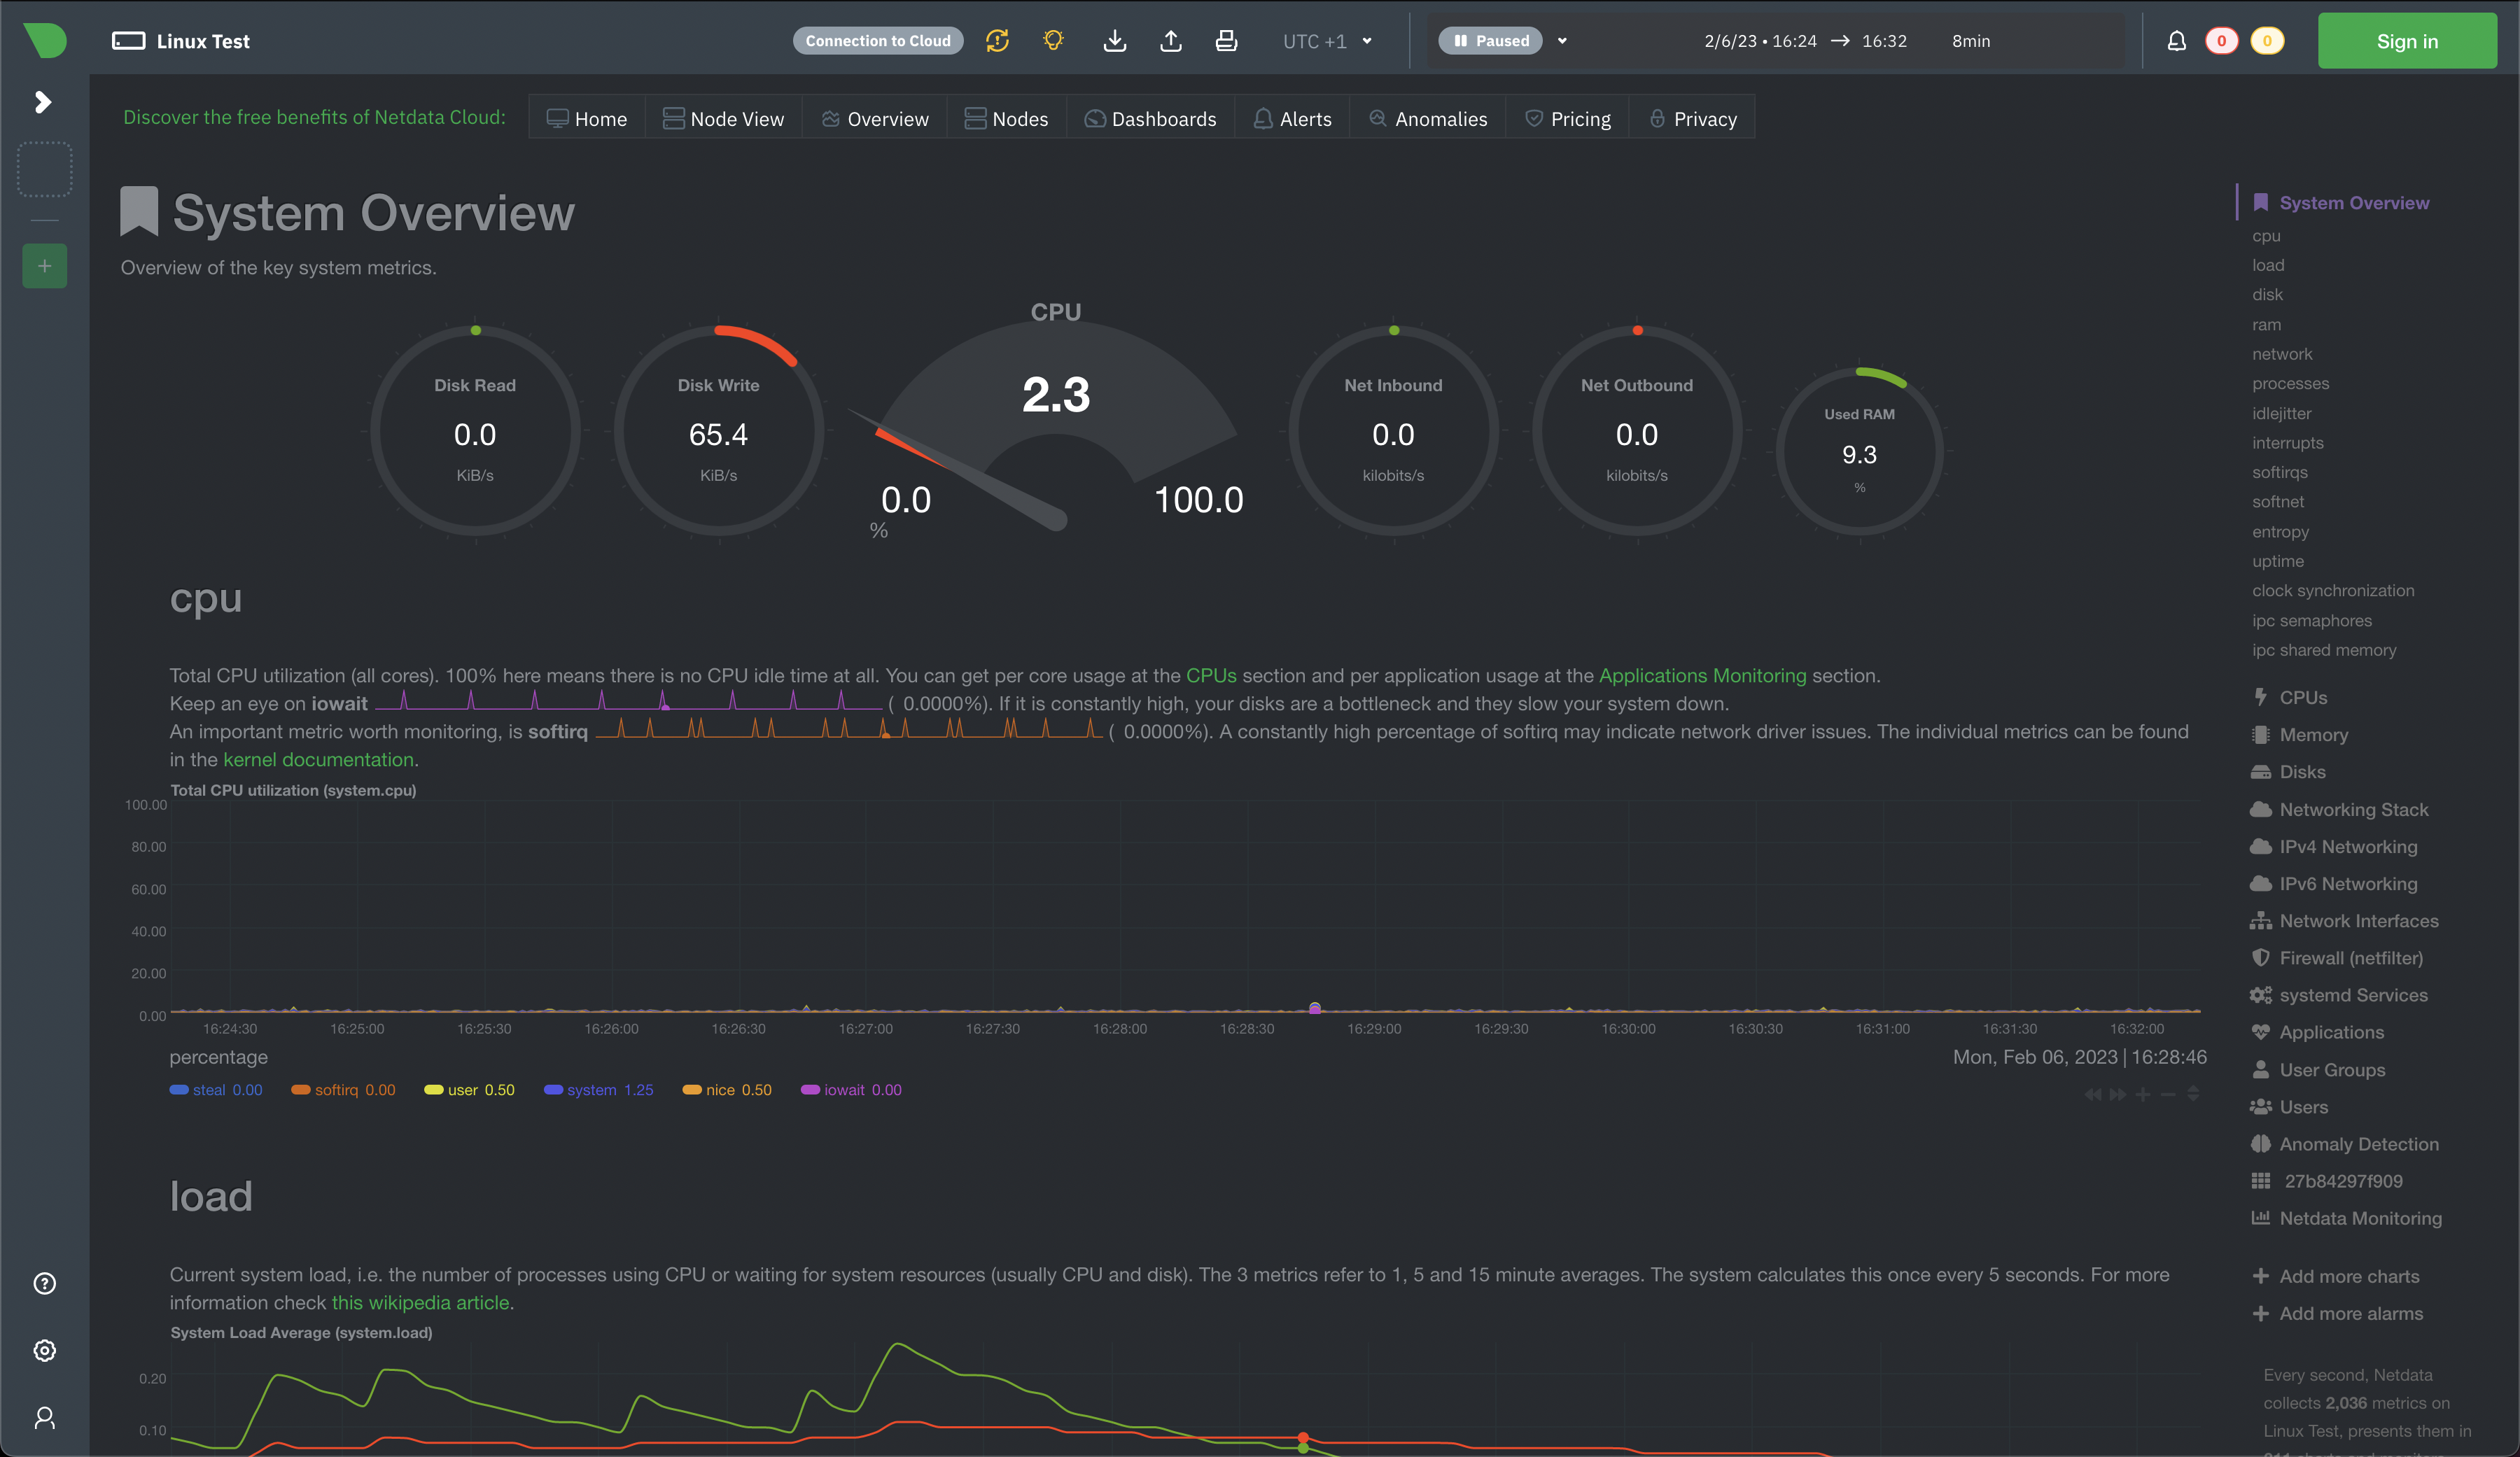
\includegraphics[width=0.95\textwidth]{figures/netdata.png}
        \caption{Netdata Dashboard Example}
        \label{fig:netdata-dashboard}
    \end{figure}
    Netdata has a vast amount of support for other tools in order to gather data. 
    One of the supported tools is \nameref{sec:prometheus-evaluation-setup}, which is used to scrape the monitored data from all resources that have Netdata installed.

  \subsection{Prometheus}
  \label{sec:prometheus-evaluation-setup}
  
    Prometheus\footnote{https://prometheus.io/} is an open source application used for monitoring and alerting of events and is designed to run across various platforms in a scalable and easily deployable manner.
    Same as Netdata it records in real-time, and stores the gathered metrics in a time series database by using a \emph{HTTP pull model}. It also allows real-time alerting via a rule defining configuration and also has a flexible query language called \emph{PromQL}, that enables the retrieval and processing the gathered data. Prometheus has great integration with other tools such as Netdata.
    In the project it is used inside a monitoring master node that is continuously scraping all resources that have Netdata installed for monitoring data. In case a predefined rule is broken at a monitored resource, such as CPU over-allocation, Prometheus triggers an event that notifies ADA-PIPE in order to be able to take measurements.



  \subsection{PyTorch}
  \label{sec:pytorch-evaluation-setup}
    PyTorch\footnote{https://pytorch.org/} is an open-source machine learning library for Python, developed by Facebook's AI Research lab (FAIR) but is now part of the \emph{Linux Foundation umbrella}. It provides tensor computation (similar to NumPy) with strong support for deep neural networks built on a tape-based autograd system. PyTorch is designed to provide flexibility and ease of use, with a focus on deep learning and neural networks. It can be used for various tasks such as natural language processing, computer vision, and speech recognition.
    PyTorch also supports deployment on various platforms, including CPUs, GPUs, and TPUs, and has an active community of users and contributors that continue to improve and expand its capabilities.
  

\section{Architecture of the Software}

  \subsection{Adaptation Loop}


  The SAA adaptation approach is defined as a loop, that cyclically updates every component contained in the loop.
  The adaptation loop is shown in figure \ref{fig:adaptation-loop} and consists of the Big Data pipeline and the \emph{resources} contain all registered and monitored to the \emph{Monitoring and Analysis} component. 
  Both the Big Data pipeline and the resources send the gathered monitoring information at a time step $P_t$ or $S_t$ respectively to the \emph{Monitoring and Analysis} component, where $t$ denotes the current time step.

  The Monitoring and Analysis component then uses the monitoring data $P_t$ and $S_t$, and calculates an action $A_{t+1}$ as an update for the resources, where $t+1$ denotes the next time step.
  
  This received action $A_{t+1}$ is then used by the Resource components to reconfigure the resources if necessary.
  The adaptation uses monitoring of tasks and resources to retrieve the monitoring data $P_t$, $S_t$.
  
  Monitoring component is necessary to obtain information about failures or performance fluctuations along with under-, over-utilization of resources.
  The monitoring data, therefore, provides feedback if a resource is able to handle additional load, and thus, more tasks will potentially be mapped to it for execution. 
  In case that the resource is not capable of handling the current load, less demanding tasks will be mapped to that resource in future scheduling cycles and it will be reconfigured accordingly.

  A monitored resource information consists of the CPU, memory and storage utilization, in addition to network bandwidth usage.
  The Big Data pipeline and resources send their monitoring data $P_t$, $S_t$ respectively to the Monitoring and Analysis component.
  Afterward, given those monitoring data, the analyzer will determine the next action $A_{t+1}$ of the resources.
  The monitoring feedback will be periodically retrieved from all registered resources and provided to the analyzer.
  In case of a resource side failure, the monitoring mechanism will be alerted of the occurred anomaly.  
  The analyzer uses this monitoring data to decide if any actions $a \in A$ on the current scheduling plan have to be applied.
  
  \begin{figure}[h!]
    \centering
     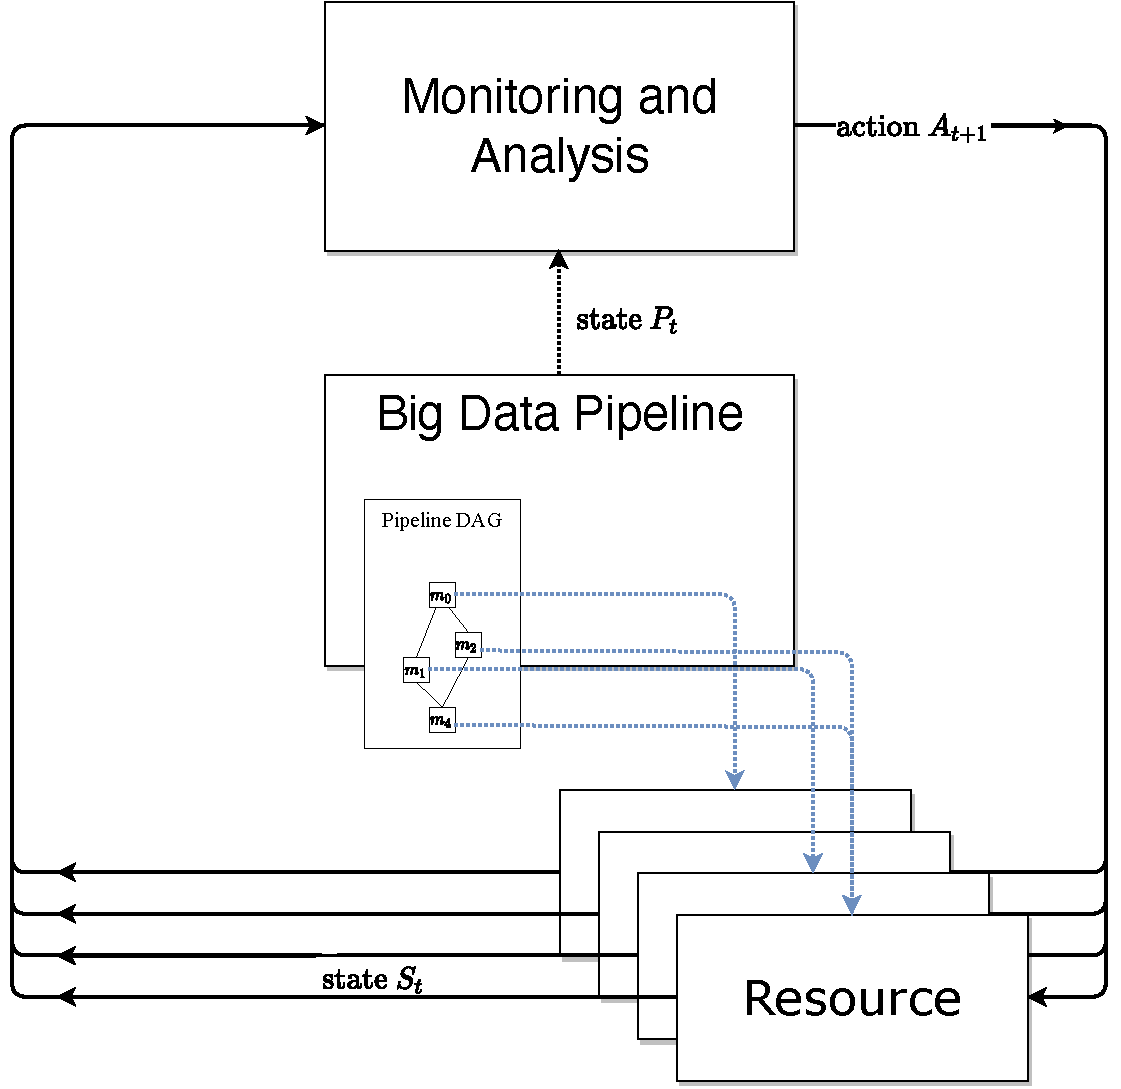
\includegraphics[width=\columnwidth]{figures/monitoring_with_inner_resources.drawio.pdf}
    \caption{Adaptation Loop}
    \label{fig:adaptation-loop}
\end{figure}
The following actions $A$ are considered in the adaptation approach:

\paragraph*{Resource load within expected parameters $(S_1)$} 
When tasks on resources are well mapped and no action has to be taken for these resources, this is denoted in the action set $A_{t+1}$ as the state $S_1$. This state is achieved when a resource is running within expected parameters, the estimated time of completing a task is not exceeded or other anomalies occur.

\paragraph*{Resource load under expected parameters $(S_2)$} 
When the monitoring component detects under-utilization of a resource, tasks of the pipeline are mapped to it to be efficiently utilized. This state is categorized as $S_2$ in the analyser and the action set will be modified to improve the utilization of resources grouped into $S_2$. 

\paragraph*{Resource load over expected parameters $(S_3)$} 
If a resource is over-utilized, there are multiple options. If it is detected that horizontal scaling solves the over-utilization and the resource instance is capable of being scaled up, it will be reconfigured to be within expected utilization levels. Furthermore, if an ill-defined task is detected and was mapped to a resource that isn't capable to fulfil the computation within a reasonable time frame, this task will be migrated to another resource. 
This is categorized as $S_3$ in the analyser, and the action set will be modified, so that resources grouped in $S_3$ will be less utilized with the upcoming updates of the action set. \cite{kimovskiBigDataPipeline2022}


\section{Monitoring}
\label{sec:monitoring-architecture}

\section{Data Preprocessing and Analysis}
\label{sec:data-preprocessing-and-analysis-architecture}

  \subsection{Feature Selection}
  \label{sec:feature-selection-data-preprocessing-architecture}

    Feature selection is the process of reducing the number of input variables of a feature set when developing a predictive model.
    Feature selection is simply the process of selecting and excluding given features without changing them as is done with \emph{dimensionality reduction}.
    A reduction of the number of input variables is desirable to both reduce reduce the computational cost of training a model and in some cases it also increases the prediction performance of the model.

    % TODO fill with more content?

  
\section{LSTM Architecture}
\label{sec:lstm-architecture-and-implementation}

  The LSTM model was implemented with \nameref{sec:pytorch-evaluation-setup}, an open-source machine learning library for Python. 
  \begin{figure}
    \centering
    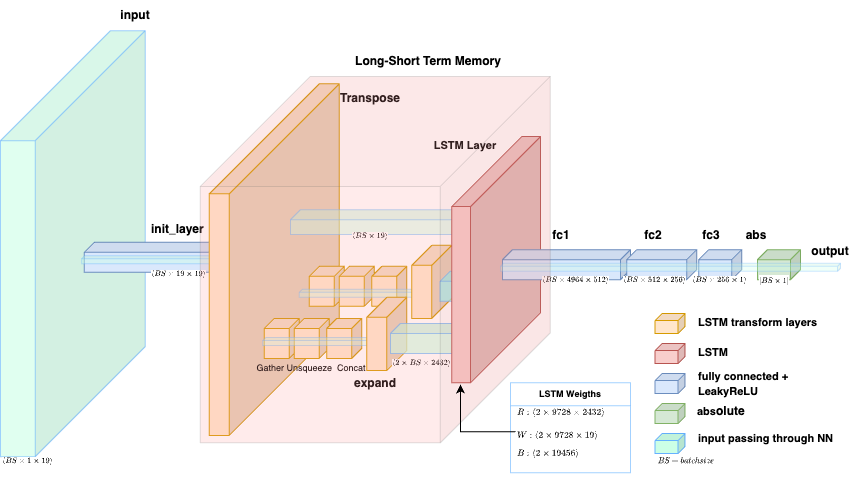
\includegraphics[scale=0.5]{figures/current_lstm_model.png}
    \caption{LSTM Model Architecture}
    \label{fig:lstm-model-architecture}
  \end{figure}

  The LSTM model implementation is called \texttt{UtilizationLSTM} and is of type \texttt{Module}. This is a default parent class for neural networks that are implemented in PyTorch.
  The class constructor \texttt{\_\_init\_\_()} has four parameters. First, is the instance reference \texttt{self} that is used to access functions and variables of an instance. 
  The available instance variables are \emph{input size, hidden size, number of layers} and \emph{device} that holds the reference to the hardware that will compute the training of the neural network.
  PyTorch enables the training of neural networks on graphical computing units (GPU) which accelerate the training process. For being able to train on a GPU, the NVIDIA API CUDA (Compute Unified Device Architecture) needs to be installed on the device, in order to send the LSTM model on the GPU and train it on incoming data batches. 
  Next, is the input size that refers to the number of feature set columns that were selected by the \nameref{sec:feature-selection-data-preprocessing-architecture} process.
  The hidden size value in the parameters also refers to the hidden layer size of the LSTM model that is used to variate the size of the model and it's capabilities to remember long-term patterns in time series data.
  Finally, the number of layers refers to how many \nameref{sec:stacked-lstm} layers should be applied.
  For the \nameref{sec:evaluation-scenarios}, a default of two stacked layers is used. When using two stacked LSTM layers, the size of the hidden layers of the model is doubled. This also includes the model output, where both hidden state outputs are returned by the \texttt{forward} function.
  The reason why an estimation that is then feed back to the model is returned is to be able to analyse the hidden states of the intermediate model layers.
  \lstinputlisting[
    language=Python, 
    caption=LSTM Init Function, 
    label={lst:lstm-init-function},
    style=codestyle
    ]{code_samples/lstm_init.py}
  Next, the two LSTM models are instantiated in lines 17 and 25 with the parameters from above. One for the prediction of CPU and one for the prediction of memory utilisation. The \texttt{batch\_first} parameter provided to both models defines how the model shall return its estimation, in this implementation, the batch will be returned first, followed by the hidden state and then the internal state.
  % TODO research if this return value is correct 
  Then, a sequential layer for both LSTM models is generated by the function shown in \ref{lst:lstm-init-sequential-layer-batchnorm}. This sequential layer consists of three components. Each component is build with the following components:
  
  \begin{pabox}{Rectified Linear Unit (ReLU)}
  \label{def:relu-definition}
    \textbf{Rectified Linear Unit (ReLU)} is a popular function for transforming the summed weighted input from a layer into the activation of a node or output for that input.
    The ReLU function can be mathematically described as $$g(z) = \max \left\{0, z\right\}.$$

  \end{pabox}
  The advantages of ReLU are it's computational simplicity, the representational sparsity (being able to output true zero values opposed to $\tanh$ and $sigmoid$), the linear behaviour and the training of deep neural networks via backpropagation was heavily improved when using ReLU compared to more complex methods. The function is linear for values greater than zero which results in ReLU having many of the advantages of a linear activation function when using backpropagation. Yet, ReLU is a nonlinear function since negative values are always output as zero.

  \begin{pabox}{Batch Normalisation}
  \label{def:batch-normalisation-definition}
    \textbf{Batch normalisation (batch norm)} is a generalisation method used to increase the stability and reduce the training time of a neural network layer by re-centering and re-scaling the inputs of the layer.
    Batch normalisation standardises the inputs to a layer for each mini-batch, and the resulting increase of stability reduces the number of required training epochs to train deep neural networks.

    \begin{quote}
      % https://machinelearningmastery.com/batch-normalization-for-training-of-deep-neural-networks/
      Batch normalization provides an elegant way of reparametrizing almost any deep network. 
      The reparametrization significantly reduces the problem of coordinating updates across many layers.
      \cite{goodfellowDeepLearning2016}
    \end{quote}
    Assumptions that a subsequent layer makes during the weight update that regards the spread and distribution of inputs, will not change by a lot if the activations of the prior layer are standardised. 
  \end{pabox}
  Normalising the input batch also has a regularising effect, which leads to a reduction of generalisation errors, similar to the usage of activation regularisation.
  Batch normalisation was proposed to mitigate internal covariate shift. This internal covariate shift occurs because inputs that are forwarded to the neural network and also from each layer have a corresponding distribution that affects the training process because of the randomness of the parameter initialisation and input data.
  Because of the resulting internal covariate shift, the succeeding network layers need to readjust it's weights in order to update it's state from the data that was forwarded from the proceeding layer with a bias in terms of distribution of activated nodes. This requirement to readjust to new distributions is even more sever in deep neural networks that have many layers and the increased number of layers amplify this effect. Batch normalisation reduces unwanted shifts that is propagated by layers and speeds up the training and also produces more reliable and general models.
  


  \begin{pabox}{Linear (Fully-Connected) Layer}
    \label{def:linear-layer-definition}
    Linear layers, also known as fully-connected layers connect every input neuron to every output neuron and are commonly used in neural networks. The structure of a neural network consisting of fully-connected layers can be seen in the figure below, where each node is connected to all nodes of the previous and the succeeding layer.
    A linear layer is defined by three parameters, the number of inputs, the number of outputs and the batch size.
    Operations such as forward propagation, activation gradient computation, and weight gradient computations are directly expressed as matrix multiplications.
    \begin{minipage}[t]{1\linewidth}
      \centering
      \vspace*{0pt}
          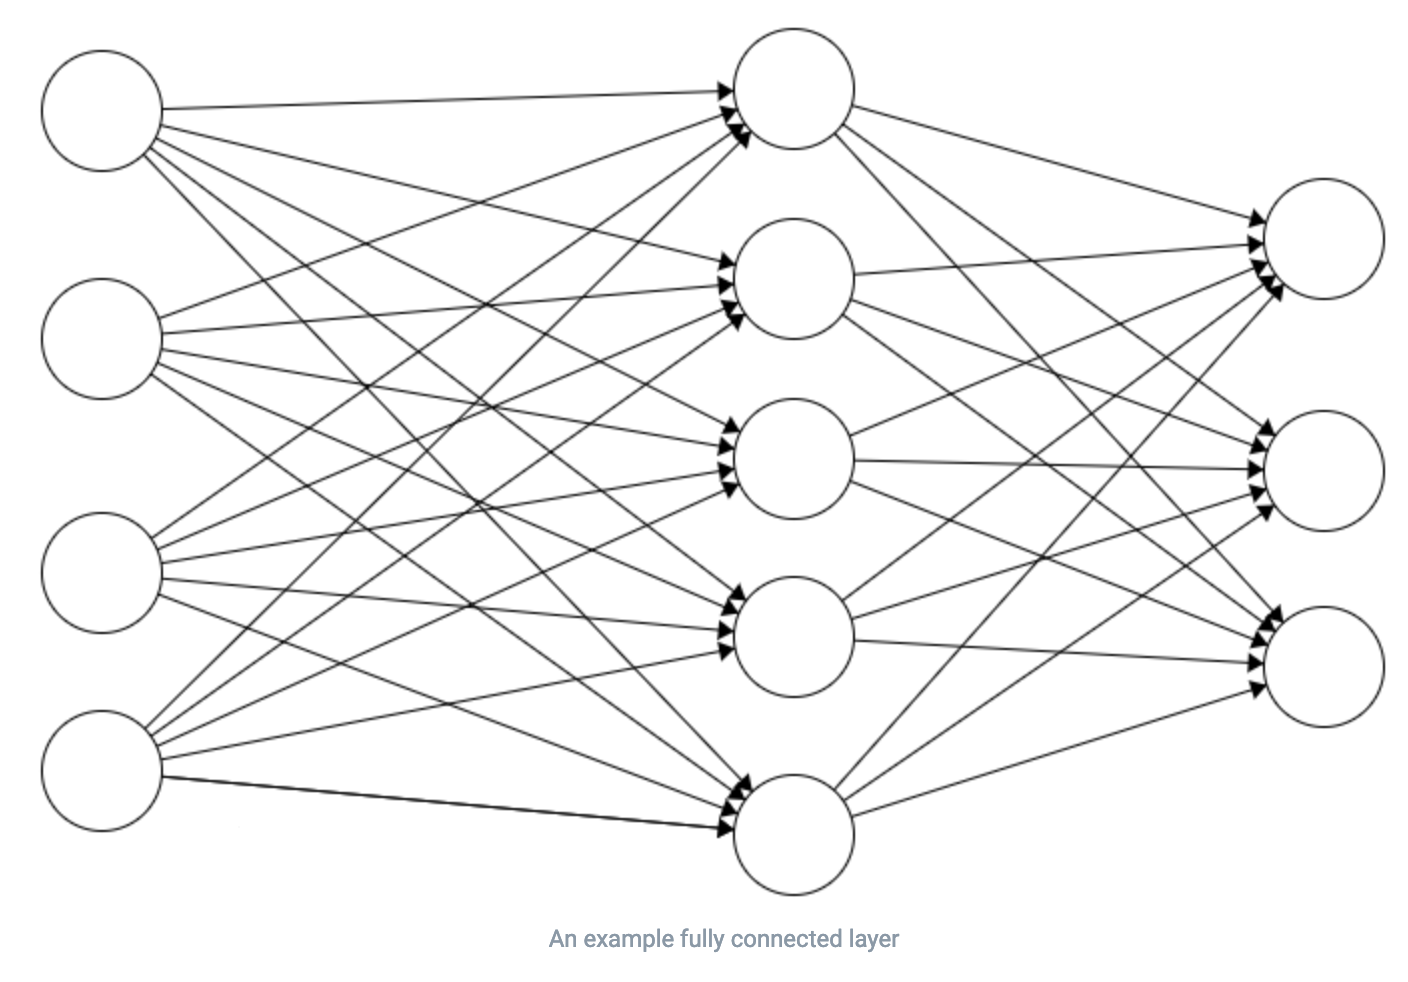
\includegraphics[height=0.25\textheight,width=0.5\linewidth]{figures/fc_layer.png}
          \captionof{figure}{Fully-Connected Layers \cite{FullyConnectedLayer}}
          \label{fig:fully-connected-layers-architecture}
          % \captionof{figure}{Misura della carica elettrica}\label{fig:fig1}
      \end{minipage}
    % A feed-forward layer is a combination of a linear layer and a bias.
    % It is capable of learning an \emph{offset} (because of the bias) and a rate of correlation (because of the linear layer).
    % While training it represents an equation of a line $y = w \times x + b$ where it tries to learn both $w$ and $b$.
  \end{pabox}
  These LSTM and sequential layers are the core of the machine learning architecture inside the \texttt{UtilizationLSTM} class and are responsible for the estimation of the CPU and memory utilisation and are used by forwarding inputs through each layer until the estimation is calculated.
  The received input is send to the \texttt{forward} function of the class that expects a PyTorch tensor as the input type.

   
  
  % TODO explain ReLU and why it is used
  \lstinputlisting[
    language=Python, 
    caption=LSTM Initialise Sequential Layers with BatchNorm, 
    label={lst:lstm-init-sequential-layer-batchnorm},
    style=codestyle
    ]{code_samples/lstm_init_seq_layer_bn.py}


  As can be seen in figure \ref{fig:lstm-model-architecture} the input vector consisting of a pipeline task batch is forwarded to the \emph{initial lstm layers}. This step is implemented in the LSTM \texttt{forward} function (see \ref{lst:lstm-forward-function}) in lines 8 and 9. The \texttt{get\_hidden\_internal\_state} (see \ref{lst:lstm-init-internal-hidden-state}) function seen on the right side of the lines 8 and 9 is used to create the initial internal and hidden state based on the time series batch provided as the \texttt{input} for the model. The input vector is a PyTorch tensor that is then send to a function that generates the initial hidden and internal state based on the shape of the input vector.
  The general LSTM prediction model is split into two smaller LSTM components that each predict the utilisation of one resource unit. A resource unit is either the CPU usage or the allocated memory. At creation these LSTM components use the length of the input as the expected input size and quality of the prediction performance heavily depends on the chosen hidden layer size as well as the number of \nameref{sec:stacked-lstm} layers.
  The final LSTM output of either resource unit is then send to traditional sequential layers that use batch normalisation as the generalisation strategy.
  % TODO describe batch normalization
  Afterwards, the output of those sequential layers is concatenated column-wise as a label vector of the form $\left[(cpu_1, mem_1), \dots, (cpu_{bs}, mem_{bs})\right]$ where $bs$ denotes the batch size or number of data points in the batch.
  At line 22 the calculated output is then sliced in order to only include the same amount of elements as are the elements of the input vector. This has to be done since using multiple LSTM layers also increases the number of output elements by the simple formula $elements_{input} \times \#layers$. For the estimation of the resource utilisation only the last estimation section of the output is required since this is the section that contains the prediction of the last LSTM layer.
  In line 25 the absolute values of the output are calculated. This is done to ensure that negative values are not included in the prediction since it is not possible for the hardware utilisation to be less than zero.
  
  % TODO Explain ReLU and other layers
  



  \lstinputlisting[
    language=Python, 
    caption=LSTM Forward Function, 
    label={lst:lstm-forward-function},
    style=codestyle
    ]{code_samples/lstm_forward.py}

  \lstinputlisting[
    language=Python, 
    caption=LSTM Initialise Internal and Hidden State, 
    label={lst:lstm-init-internal-hidden-state},
    style=codestyle
    ]{code_samples/lstm_get_hidden_int_state.py}



  

\section{Adaptation}
  \subsection{Resource Prediction}
  % flow chart of resource prediction
  \subsection{DataFrame Scaler}
  \subsection{Penalty Mean Squared Error Loss Function}
  \label{sec:penalty-mse-loss-function-architecture-and-implementation}

    The \emph{Penalty Mean Squared Error (PMSE) loss function} is a custom loss function based on the commonly used \emph{Mean Squared Error (MSE) loss function} \cite{koksoyMultiresponseRobustDesign2006} (see \ref{def:mean-squared-error-definition}). 
    
    The Mean Squared Error metric measures how close a \nameref{sec:regression-supervised-learning-background} line is to a set of data points. It is a risk function that corresponds to the expected value $y_i$ fo the squared error loss (see \ref{fig:regression-example}). A larger MSE indicates that the data points are widely dispersed around its mean, where a smaller MSE indicates the opposite.

    \begin{pabox}{Mean Squared Error}
    \label{def:mean-squared-error-definition}
      The \emph{Mean Squared Error (MSE)} of an estimator (i.e. trained LSTM model) measures the average of the squares of the errors, which is the average squared difference between the actual value $y$ and the estimated values $\hat{y}$.

      $$MSE = \frac{1}{N} \sum_{i = 1}^{N}\left(y_i - \hat{y}_i\right)^2$$

      The squaring is critical to reduce the complexity with negative signs. If used as a loss function (criterion), the machine learning algorithm will update it's weights in order to reduce the calculated loss value produced by the MSE loss function.
    \end{pabox}

    Penalty in this loss function refers to increasing the loss of predicted values $\hat{y}_i$ that are lower than the actual value $y_i$.

    \begin{pabox}{Calculation of the Penalised Prediction Value $\hat{y'}_i$}
    \label{def:calculation-of-the-penalty-value}

      The penalty is defined as a positive real number ranging from zero to infinity and it's mathematical representation is $Penalty = [0, \infty]$.
      The penalty value denoted as $Penalty$ is subtracted from a predicted value $\hat{y}_i$ if it is smaller than the actual value $y_i$. A subtraction is required to further increase the distance between the actual value and the (under-allocated) predicted value.
      The result of this calculation is the updated penalised prediction value $\hat{y'}_i$.
      This conditional mathematical representation is shown in the following:
      $$\hat{y'}_i = 
      \begin{cases}
        \hat{y}_i - Penalty, & \quad \textrm{if } \hat{y}_i < y_i \\
        \hat{y}_i,  & \quad \textrm{otherwise}
      \end{cases}$$
      Therefore, the more the prediction values are below the actual values, the more the penalty value is applied, and thus the error of a predicted data batch increases.

    \end{pabox}

    The custom PMSE was implemented because the more information was included in the feature set while training, the more likely the LSTM model is to predict values that are lower than the actual value (see \nameref{sec:evaluation-scenarios}). Since an estimation lower than the actual value could lead to problems such as a task not finishing in the required time frame, or an \emph{out of memory} exception, that not only interrupts the system to terminate the task, but could also lead to system failure. This is the reason why a penalty is added to the predicted value in case of being lower than the actual value. With this measure in place, the LSTM model is more likely to predict values that are higher than the actual value. While this might introduce resource wastage, it is still preferable to introduce some resource wastage than providing an unstable system configuration.

    \begin{pabox}{Penalty Mean Squared Error}
      \label{def:penalty-mean-squared-error-definition}
      The \emph{Penalty Mean Squared Error (PMSE)} of an estimator (i.e. trained LSTM model) measures the average of the squares of errors similar to \emph{mean squared error} but also applies a penalty to estimated values $\hat{y}_i$ that are lower than the actual value $y_i$ (see \ref{def:calculation-of-the-penalty-value}). 
      The mathematical representation of PMSE is:
      $$PMSE = \frac{1}{N} \sum_{i = 1}^{N}\left(y_i - \hat{y'}_i\right)^2$$
      As can be seen, it is similar to the representation of MSE (see \ref{def:mean-squared-error-definition}), but uses a modified estimated value $\hat{y'}_i$ that was penalised before the calculation.
    \end{pabox}

    The \texttt{PenaltyMSELoss} class inherits from the PyTorch Module package in order to be able to use it as the loss function for the error calculation of the predicted and actual values.
    The \texttt{PenaltyMSELoss} class constructor (see listing \ref{lst:pmse-python-class} line 4) has two parameters, the \texttt{self} keyword that is used to access instance parameters, and the \texttt{penalty} parameter, that is expected to be of type \texttt{float}.
    Inside the class constructor, a \texttt{MSELoss} instance (line 6) will be created in order to calculate the final loss values based on the mean square error calculation.

    The \texttt{forward} function (see \ref{lst:pmse-python-class} line 9) is used to calculate the loss between the estimation (denoted as \texttt{pred}) and actual values (denoted as \texttt{actual}). Both the estimation and actual values are represented as PyTorch tensors, a multi-dimensional matrix that contains the elements of a single data type, in this case floating point numbers.
    The function also expects its calculated output to be of type \texttt{float}, which is a common data type for loss functions.
    In line 10 the indices of all predictions smaller than the actual values that would result in an under-allocation of resources are stored in a \texttt{boolean} array.
    This array is then used in line 11 to update all values that match the indices stored in the array by subtracting the penalty value.
    After updating all predicted values both tensors are then forwarded to the mean squared error function in line 13, that does the final calculation of the loss.
    The MSE function then returns the value to the calling function \texttt{forward} and this returns the loss value as type \texttt{float}.

    \lstinputlisting[
      language=Python, 
      caption=Penalty Mean Squared Error Python Class, 
      label={lst:pmse-python-class},
      style=codestyle
      ]{code_samples/pmse.py}


